%% LaTeX-Beamer template for KIT design
%% by Erik Burger, Christian Hammer
%% title picture by Klaus Krogmann
%%
%% version 2.1
%%
%% mostly compatible to KIT corporate design v2.0
%% http://intranet.kit.edu/gestaltungsrichtlinien.php
%%
%% Problems, bugs and comments to
%% burger@kit.edu

\documentclass[18pt]{beamer}
\usepackage[utf8x]{inputenc}
\usepackage{units}
\usepackage{booktabs}

%% CUSTOM
\usepackage{amsmath}
\usepackage{algpseudocode}

%% Definitions
\DeclareMathOperator{\div2}{div}
\renewcommand{\algorithmicrequire}{\textbf{Input:}}
\renewcommand{\algorithmicensure}{\textbf{Output:}}
\algnewcommand\algorithmicto{\textbf{to}}
\algrenewtext{For}[3]{\algorithmicfor\ $#1 \gets #2$ \algorithmicto\ $#3$ \algorithmicdo}
\algnewcommand\algorithmicod{\textbf{od}}
\algrenewtext{EndWhile}{\algorithmicod}
\algrenewtext{EndFor}{\algorithmicod}
%\AtBeginSection[]{%
%\begin{frame}<beamer> % do nothing in handouts
%    \frametitle{Überblick}
%    \tableofcontents[sectionstyle=show/shaded,
%    subsectionstyle=show/show/hide]
%\end{frame}
%}
%\AtBeginSubsection[]{%
%\begin{frame}<beamer> % do nothing in handouts
%    \frametitle{Überblick}
%    \tableofcontents[sectionstyle=show/shaded,
%    subsectionstyle=show/shaded/hide]
%\end{frame}
%}

%% SLIDE FORMAT

% use 'beamerthemekit' for standard 4:3 ratio
% for widescreen slides (16:9), use 'beamerthemekitwide'

\usepackage{templates/beamerthemekit}
%\usepackage{templates/beamerthemekitwide}

 %% TITLE PICTURE

 % if a custom picture is to be used on the title page, copy it into the 'logos'
 % directory, in the line below, replace 'mypicture' with the 
 % filename (without extension) and uncomment the following line
 % (picture proportions: 63 : 20 for standard, 169 : 40 for wide
 % *.eps format if you use latex+dvips+ps2pdf, 
 % *.jpg/*.png/*.pdf if you use pdflatex)


 \titleimage{banner}
 
 
%% Define some colors:
\definecolor{darkblue}{rgb}{0,0,.5}
\definecolor{darkgreen}{rgb}{0,.5,0}

 %% TITLE LOGO

 % for a custom logo on the front page, copy your file into the 'logos'
 % directory, insert the filename in the line below and uncomment it

\titlelogo{logo_150x150}
 
 % (*.eps format if you use latex+dvips+ps2pdf,
 % *.jpg/*.png/*.pdf if you use pdflatex)
 
 %% TikZ INTEGRATION
 
 % use these packages for PCM symbols and UML classes
 % \usepackage{templates/tikzkit}
 % \usepackage{templates/tikzuml}
 
 % the presentation starts here
 
\author{Dominik Muth - dominik.muth@student.kit.edu}
\institute{Institut f\"ur Informatik}

\subtitle{Foliensatz 10}
\date{10. Januar 2013}

\begin{document}

\begin{frame}
    \titlepage
\end{frame}

\begin{frame}{Outline/Gliederung}
    \tableofcontents
\end{frame}

\section{Master-Theorem}
\begin{frame}{Master-Theorem}
    \begin{block}{Definition}
        Für einen \emph{rekursiven} Algorithmus der Form
        \begin{align*}
            T\left( n \right) = aT\left( \frac{n}{b} \right) + f\left( n \right)
        \end{align*}
        kann die Laufzeit für drei Fälle abgeschätzt werden:
        \pause
        \begin{enumerate}
            \item Wenn $f\left( n \right)\n \mathcal{O}\left( n^{\log_b a-\varepsilon} \right)$ für ein $\varepsilon > 0$, dann ist $T\left( n \right) \in \Theta\left( n^\log_b a \right)$
                \pause
            \item Wenn $f\left( n \right)\n \Theta\left( n^{\log_b a} \right)$, dann ist $T\left( n \right) \in \Theta\left( n^\log_b a \log n\right)$
                \pause
            \item Wenn $f\left( n \right)\n \Omega\left( n^{\log_b a+\varepsilon} \right)$ für ein $\varepsilon > 0$, \\ und wenn es eine Konstante $d$ gibt mit $0<d<1$,\\ sodass für alle hinreichend großen $n$ gilt $af\left( \nicefrac{n}{b} \right) \leq df\left( n \right)$,\\ dann ist $T\left( n \right) \in \Theta\left( f\left( n \right) \right)$
        \end{enumerate}
    \end{block}
    \begin{itemize}
        \item Fall 2 wird etwa bei Quicksort benötigt
        \item Fall 3 ist eher die Ausnahme
    \end{itemize}
\end{frame}

\section{Mealy-Automat}
\begin{frame}{Mealy-Automat}
    \begin{block}{Definition: Mealy-Automat}
        Der Mealy-Automat $A = \left( Z, z_0, X, f, Y, g \right)$ besteht aus
        \begin{enumerate}
            \item der endlichen Zustandsmenge $\mathbf{Z}$,
            \item dem Startzustand $\mathbf{z_0}$,
            \item dem Eingabealphabet $\mathbf{X}$,
            \item der Zustandsübergangsfunktion $\mathbf{f: Z\times X \rightarrow Z}$,
            \item einem Ausgabealphabet $\mathbf{Y}$ und
            \item der Ausgabefunktion $\mathbf{g: Z\times X \rightarrow Y^*}$.
        \end{enumerate}
    \end{block}
\end{frame}
\begin{frame}{Getränkeautomat}
    \begin{figure}[htbp]
        \centering
        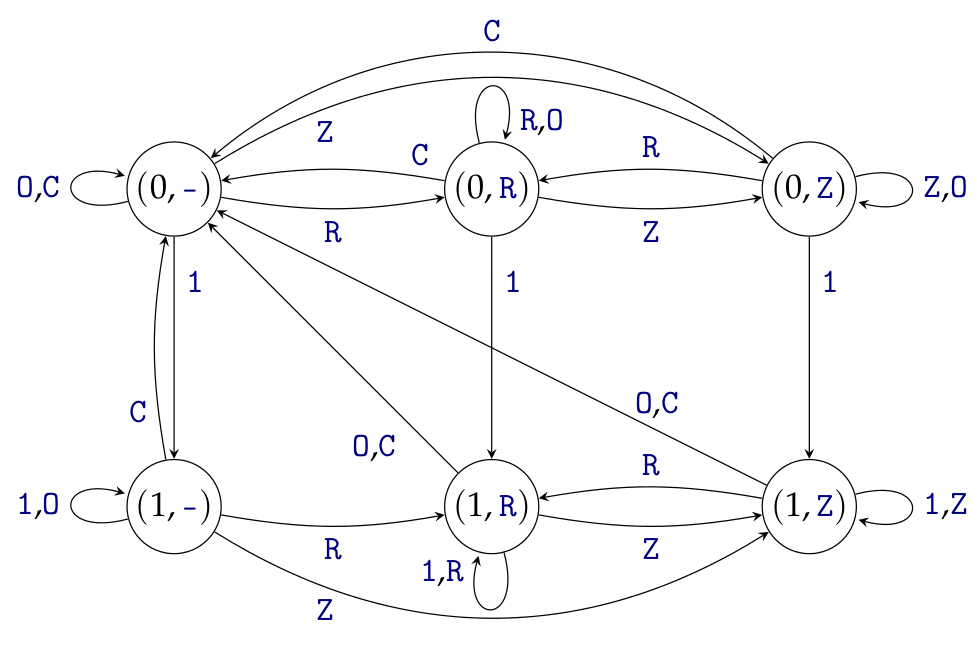
\includegraphics[width=\textwidth,height=\textheight,keepaspectratio]{graphics/10/getraenke.png}
    \end{figure}
\end{frame}
\begin{frame}{Getränkeautomat}
    Was ist was?
    \begin{itemize}
        \item Zustandsmenge $Z$: $\left\{ \left( 0,- \right), \left( 0,R \right), \left( 0,Z \right), \left( 1,- \right), \left( 1,R \right), \left( 1,Z \right) \right\}$
    \end{itemize}
\end{frame}

\section{Moore-Automat}

\section{Endliche Akzeptoren}
\end{document}
